\documentclass{beamer}
\setbeamertemplate{footline}[page number]
\date{}
\author{}
\institute{}

%%%%%%% Put these names back in the final version 
%\\Aswathy Rajendra Kurup\\Meenu Ajith}
%\institute{Department of Electrical and Computer Engineering\\The University of New Mexico}
\setbeamercovered{transparent}
\usepackage{setspace}
\usepackage{array}
\usepackage[T1]{fontenc}
\usepackage{graphicx}
\usepackage{amsmath}
\usepackage{amsfonts}
\usepackage{amssymb}
\usepackage{makeidx}
\usefonttheme{serif}
\usepackage{multirow}
\usepackage{booktabs} 
\usepackage{rotating}
\usepackage{color}
\usepackage{float}
\usepackage[latin1]{inputenc}
\usepackage[english]{babel}
\usepackage{amsmath}
\usepackage{amsfonts}
\usepackage{eurosym}
\usepackage{rotating}
\usepackage{multicol}
\usepackage{pythonhighlight}
\usepackage[normalem]{ulem}
\newcommand{\ba}{{\bf a}}
\newcommand{\bb}{{\bf b}}
\newcommand{\bc}{{\bf c}}
\newcommand{\bd}{{\bf d}}
\newcommand{\be}{{\bf e}}
\newcommand{\bbf}{{\bf f}}
\newcommand{\bg}{{\bf g}}
\newcommand{\bh}{{\bf h}}
\newcommand{\bi}{{\bf i}}
\newcommand{\bk}{{\bf k}}
\newcommand{\bl}{{\bf l}}
\newcommand{\bm}{{\bf m}}
\newcommand{\bn}{{\bf n}}
\newcommand{\bo}{{\bf o}}
\newcommand{\bp}{{\bf p}}
\newcommand{\bq}{{\bf q}}
\newcommand{\br}{{\bf r}}
\newcommand{\bs}{{\bf s}}
\newcommand{\bt}{{\bf t}}
\newcommand{\bu}{{\bf u}}
\newcommand{\bv}{{\bf v}}
\newcommand{\bw}{{\bf w}}
\newcommand{\bx}{{\bf x}}
\newcommand{\by}{{\bf y}}
\newcommand{\bz}{{\bf z}}

\newcommand{\bA}{{\bf A}}
\newcommand{\bB}{{\bf B}}
\newcommand{\bC}{{\bf C}}
\newcommand{\bE}{{\bf E}}
\newcommand{\bG}{{\bf G}}
\newcommand{\bH}{{\bf H}}
\newcommand{\bI}{{\bf I}}
\newcommand{\bK}{{\bf K}}
\newcommand{\bL}{{\bf L}}
\newcommand{\bM}{{\bf M}}
\newcommand{\bO}{{\bf O}}
\newcommand{\bQ}{{\bf Q}}
\newcommand{\bR}{{\bf R}}
\newcommand{\bS}{{\bf S}}
\newcommand{\bT}{{\bf T}}
\newcommand{\bV}{{\bf V}}
\newcommand{\bW}{{\bf W}}
\newcommand{\bX}{{\bf X}}
\newcommand{\bY}{{\bf Y}}
\newcommand{\bZ}{{\bf Z}}
\newcommand\uptocnt{\stackrel{\mathclap{\normalfont\mbox{c}}}{\propto}}
\newcommand{\bpt}{{\bf pt}}
\newcommand{\bpl}{{\bf pl}}
\newcommand{\bdp}{{\bf dp}}
\newcommand{\btemp}{{\bf temp}}

\newcommand{\bmu}{{\boldsymbol \mu}}
\newcommand{\bSigma}{{\boldsymbol \Sigma}}
\newcommand{\bsigma}{{\boldsymbol \sigma}}
\newcommand{\bvarPhi}{{\boldsymbol \varPhi}}
\newcommand{\bvarphi}{{\boldsymbol \varphi}}
\newcommand{\bPhi}{{\boldsymbol \Phi}}
\newcommand{\bdelta}{{\boldsymbol \delta}}
\newcommand{\bZero}{{\bf 0}}
\newcommand{\bOne}{{\bf 1}}
\newcommand{\balpha}{{\boldsymbol \alpha}}
\newcommand{\bAlpha}{{\boldsymbol A}}
\newcommand{\btheta}{{\boldsymbol \theta}}

\newcommand{\softmax}{\text{softmax}}
\newcommand{\diag}{\text{diag}}
\newcommand{\sinc}{\mathrm{sinc}}
\newcommand{\argmin}{\mathop{\mathrm{argmin}}}
\newcommand{\infl}{\eta}
\newcommand{\Ind}{\mathrm{I}}
\newcommand{\Real}{\mathbb R}
\newcommand{\Intg}{\mathbb Z}
\newcommand{\Complex}{\mathbb C}
\newcommand{\Natural}{\mathbb N}
\newcommand{\Fourier}[1]{\mathcal{F} \{#1\}}
%\newcommand{\ii}{\mathbbm{i}}
\newcommand{\bphi}{\boldsymbol{\mathit{\phi}}}

\newcommand{\hs}{\hspace{2pt}}
\newcommand{\sign}{\text{sign}}
\author{Manel Mart\'inez-Ram\'on\\Meenu Ajith\\Aswathy Rajendra Kurup}

\usetheme{Madrid}
\usecolortheme{beaver}
\usepackage{tikz}
\usetikzlibrary{fit,arrows,calc,positioning}
\usepackage{listings}
\usepackage{xcolor}
\usepackage{emerald} 
\usepackage[T1]{fontenc} 
\usepackage{verbatim}
\usepackage{graphicx}
\usepackage{epsfig}
\usepackage{psfrag}
\usepackage[english]{babel}
\usepackage{listings}
\usepackage{courier}
\usepackage{color}
 \usepackage{vwcol} 
 \usepackage[english]{babel} % To obtain English text with the blindtext package
\usepackage{blindtext}
\definecolor{codegreen}{rgb}{0,0.6,0}
\definecolor{codegray}{rgb}{0.5,0.5,0.5}
\definecolor{codepurple}{rgb}{0.58,0,0.82}
\definecolor{backcolour}{rgb}{0.95,0.95,0.92}

\lstdefinestyle{mystyle}{
  backgroundcolor=\color{backcolour},   commentstyle=\color{codegreen},
  keywordstyle=\color{magenta},
  numberstyle=\tiny\color{codegray},
  stringstyle=\color{codepurple},
  basicstyle=\ttfamily\footnotesize,
  breakatwhitespace=false,         
  breaklines=true,                 
  captionpos=b,                    
  keepspaces=true,                 
  numbers=left,                    
  numbersep=5pt,                  
  showspaces=false,                
  showstringspaces=false,
  showtabs=false,                  
  tabsize=2
}
\lstset{style=mystyle}

%% Stuff for movies

% %\newcommand{\bt}{{\bf t}}
% \newcommand{\br}{{\bf r}}
% \newcommand{\bs}{{\bf s}}
% \newcommand{\by}{{\bf y}}
% \newcommand{\bz}{{\bf z}}
% \newcommand{\bx}{{\bf x}}
% \newcommand{\bw}{{\bf w}}
% \newcommand{\be}{{\bf e}}
% \newcommand{\bbf}{{\bf f}}
% \newcommand{\bb}{{\bf b}}
% \newcommand{\bd}{{\bf d}}
% \newcommand{\bA}{{\bf A}}
% \newcommand{\bB}{{\bf B}}
% \newcommand{\bL}{{\bf L}}
% \newcommand{\bM}{{\bf M}}

% \newcommand{\bC}{{\bf C}}
% \newcommand{\bI}{{\bf I}}
% \newcommand{\bK}{{\bf K}}
% \newcommand{\bk}{{\bf k}}
% \newcommand{\bT}{{\bf T}}
% \newcommand{\bV}{{\bf V}}
% \newcommand{\bW}{{\bf W}}
% \newcommand{\bX}{{\bf X}}
% \newcommand{\bY}{{\bf Y}}
% \newcommand{\bZ}{{\bf Z}}
% \newcommand{\bm}{{\bf m}}
% \newcommand{\bpt}{{\bf pt}}
% \newcommand{\bpl}{{\bf pl}}
% \newcommand{\bdp}{{\bf dp}}
% \newcommand{\btemp}{{\bf temp}}
% \newcommand{\bl}{{\bf l}}
% \newcommand{\bu}{{\bf u}}
% \newcommand{\bmu}{{\boldsymbol \mu}}
% \newcommand{\bSigma}{{\boldsymbol \Sigma}}
% \newcommand{\bLambda}{{\boldsymbol \Lambda}}

% \newcommand{\bsigma}{{\boldsymbol \sigma}}
% \newcommand{\bvarphi}{{\boldsymbol \varPhi}}
% \newcommand{\btheta}{{\boldsymbol \theta}}
% \newcommand{\bZero}{{\bf 0}}
% \newcommand{\balpha}{{\boldsymbol \alpha}}
% \newcommand{\bpi}{{\boldsymbol \pi}}
% \newcommand{\bxi}{{\boldsymbol \xi}}
% \newcommand{\bdelta}{{\boldsymbol \delta}}
\lstset{
	language=Python,
	basicstyle=\footnotesize\ttfamily\color{black},
	commentstyle = \footnotesize\ttfamily\color{red},
	keywordstyle=\footnotesize\ttfamily\color{blue},
	stringstyle=\footnotesize\ttfamily\color{black},
%	columns=fixed,
%	numbers=left,    
	numberstyle=\tiny,
	stepnumber=1,
	numbersep=5pt,
	tabsize=1,
	extendedchars=true,
	breaklines=true,            
	frame=b,         
	showspaces=false,
	showtabs=true,
	xleftmargin=6pt,
	framexleftmargin=6pt,
	framexrightmargin=2pt,
	framexbottommargin=4pt,
	showstringspaces=false      
}

\lstloadlanguages{
         Python
}

%\graphicspath{ {./images/} }  % Figures path - used in graphicx

%\selectcolormodel{cmyk}

\mode<presentation>

\newcommand{\dred}{darkred!90!black}
\newcommand{\written}{\ECFJD\textcolor{cyan!50!white}}
\newcommand{\hlight}{\textcolor{\dred}}
\newcommand{\Ex}{\textcolor{\dred}{Ex. }}

% remove navigation symbols in full screen mode
\setbeamertemplate{navigation symbols}{}  
\setbeamertemplate{blocks}[rounded][shadow=false]
\setbeamercolor{note page}{fg=black}

\setbeamercolor{title}{fg=\dred}
\setbeamercolor{frametitle}{fg=white}
\setbeamercolor{frametitle}{bg=\dred}
\setbeamercolor{structure}{fg=black,bg=white}
\setbeamercolor{background canvas}{bg=white,fg=black}
\setbeamercolor{normal text}{fg=black,bg=white}
\setbeamercolor{item}{fg=red!80!black,bg=white!}
\addtobeamertemplate{block begin}{\setbeamercolor{block title}{fg=white,bg=\dred}
\setbeamercolor{block body}{fg=white,bg=gray}}{}


\title{6. Attention-based networks}
\subtitle{6.3. Transformers for vision}

\addtobeamertemplate{frametitle}{}


\begin{document}
\maketitle


\begin{frame}{Introduction}
\begin{itemize}

\item Transformers were initially developed for natural language processing (NLP), with impressive performance in machine translation and text generation.

\item Also recently applied to computer vision tasks as image classification, object detection, semantic segmentation, and others.

\item Transformers can potentially overcome some of the limitations of traditional CNNs, such as limited ability to handle long-range dependencies and global context.

\item Recent advancements have paved the way for developing models that capture local and global features while handling large variations in object scales and spatial configurations.


\end{itemize}
\end{frame}

\begin{frame}{Introduction}

    \begin{itemize}
        \item Convolution can be replaced with self-attention
        \item Self-attention can learn to behave similarly to convolution.
        \item If no constraints in patch size are applied, vision transformers can extract patches from images and use to encode them. 
        \item Transformers show better scalability than convolutions. 
        \item They outperform ResNets. 
    \end{itemize}
\end{frame}

\begin{frame}{Vision transformer}{Structure}
\vspace{-0.6cm}
\begin{center}
    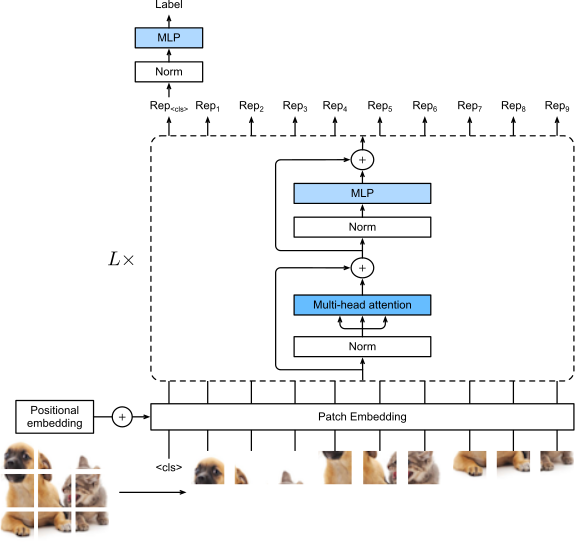
\includegraphics[scale=0.43]{Module 6 (Attention-based networks)/pics/vit.pdf}
\end{center}
\end{frame}

\begin{frame}{Vision transformer}{Operation}

\begin{itemize}
\item Images as tokens:
\begin{itemize}
\item Input image with height $h$, width $w$, and $C$
 channels. 
 \item patch size with dimension $p$
\item The image is split into a sequence of $m=hw/p^2$
 flattened patches with length $Cp^2$
 \item  A special <cls> (class) token.
\end{itemize}

\item Sequences are added to learnable positional encodings
\item The transformer produces $m$  output vector representations of the same length. 

\item The <cls> token attends to all the image patches via self-attention. Its representation from the Transformer encoder output is transformed into the output label.
\end{itemize}   

\end{frame}
\begin{frame}{Vision transformer}{Operation}
\begin{itemize}
    \item The transformer consists of alternating multi-head attention and MLP blocks. 
    \item The first layer is a 
\begin{equation}
   \bz_0 = \left[\bx_{class},  \bE\bx_1, \cdots, \bE\bx_n  \right] + \bE_{pos}
\end{equation}
where $\bx_n$ is a patch of the image, $\bE$ is an embedding matrix and $\bE_{pos}$ is a positional embedding

\item The expression of the next layers are
\begin{equation}
\begin{split}
     \bz'_{l}&=\text{MSA}\left((\text{LN}\left(\bz_{l-1}\right)\right)+\bz_{l-1}\\
     \bz_l&=\text{MLP}(\text{LN}(\bz_{l}))+\bz'_{l}
\end{split}
\end{equation}
where MSA stands for multihead self-attention and LN is layer normalization. 
\end{itemize}
\end{frame}
\begin{frame}{Vision transformer}{Operation}
    \begin{itemize}
        \item The MLP has two layers and Gaussian Error Linear Activation (GELU)
        \end{itemize}
\begin{equation}
      \text{GELU}(u) =  x \varPhi(u) \approx 0.5 x\left(1 + \tanh\left[\sqrt{\frac{2}{\pi}}\left(x+0.044715x^3 \right)\right]\right)
\end{equation}
      where $\varPhi$ is the error function.


\begin{multicols}{2}
    
    \includegraphics[scale=0.3]{Module 6 (Attention-based networks)/pics/GELU.pdf}

\columnbreak

The first element of the sequence at the output is used to code the image class 
\begin{equation}
    \by = \text{LN}\left( \bz_L^0 \right)
\end{equation}

\end{multicols}
The input sequence can be constructed from feature maps of a CNN.
\end{frame}

\begin{frame}{Vision transformer Experiments}{Datasets}
\begin{itemize}
\item Training 
\begin{itemize}
    \item ILSVRC-2012 ImageNet dataset with 1000 classes nd  1.3M  images.
    \item ImageNet-21k  with 21000 classes and 14M images 
    \item JFT  with 18000 classes and 303M high-resolution images.  
    
    
\end{itemize}
\item Test
\begin{itemize}
\item  ImageNet with original validation labels 
\item ImageNet with  ReaL labels 
\item CIFAR-10/100 
\item Oxford-IIIT Pets
\item Oxford Flowers-102 
\item VTAB
\end{itemize}
\end{itemize}
\end{frame}

\begin{frame}{Models and results}
    \begin{table}[]
\begin{tabular}{lccccc}
Model     & layers & Hidden size D & MLP size & Heads & Parameters \\ \hline
ViT-Base  & 12     & 768           & 3072     & 12    & 86M        \\
ViT-Large & 24     & 1024          & 4096     & 12    & 307M       \\
ViT-Huge  & 32     & 1280          & 5120     & 16    & 632M       \\ \hline
\end{tabular}
\end{table}
\begin{center}
    \includegraphics[scale=0.18]{Module 6 (Attention-based networks)/pics/resultsViT.png}
\end{center}
14 and 16 stand for the patch size. First L model trained with JFT and second L model trained with Imagenet21K. 
\end{frame}
\end{document}


